\documentclass{cshonours}
\bibliographystyle{acm}

\usepackage{graphics}  %optional

\title{RNA Folding: Local Versus Global Optimization}
\author{Max Ward (20748588)}

\keywords{Honours, report, dissertation, UWA, RNA, bioinformatics}
\categories{Not, really, sure}

\begin{document}
\maketitle

\begin{abstract}
I am definitely going to need to write this at some point. This is a short report on how to use the {\tt cshonours.cls} class
to prepare dissertations using the latest \LaTeX\ version,
\LaTeX2e. This class is based on the standard class {\tt report.cls}.
\end{abstract}

\begin{acknowledgements}
Going to need something here too.
This class is designed to produce reports that look
the same as those produced by the older {\tt cshonours.sty} style for
\LaTeX 2.09, which was modified by Nick Spadaccini from a style
provided by Ken Wessen.
\end{acknowledgements}

\tableofcontents
\listoftables  %optional
\listoffigures  %optional



\chapter{Introduction}
\section{DNA and RNA}
Deoxyribonucleic Acid (DNA) is the basic genetic building block upon which the classification of genetic material into genes and chromosomes is based. The role of DNA as the hereditary unit of genetics was determined in the 1940s \cite{albertsessential}. Soon thereafter, Watson \& Crick \cite{watson1953molecular} published a highly acclaimed paper describing the fundamental chemical structure of DNA. In it, they outlined a double helix formation which has since become as iconic as it is canonical (see Figure \ref{dna}). Each strand of the helix Watson \& Crick discovered is essentially a chain of `nucleotides' which are made of a sugar-phosphate backbone, attached to a single `base'. The bases of each strand form hydrogen bonds which hold the double helix together. The most astonishing and important of their findings was that these bases bond in a reciprocal fashion. They described four bases: Adenine (A), which always bonds to Thymine (T), and Guanine (G), which always bonds to Cytosine (C).

\begin{figure}
\begin{center}
\scalebox{0.23}{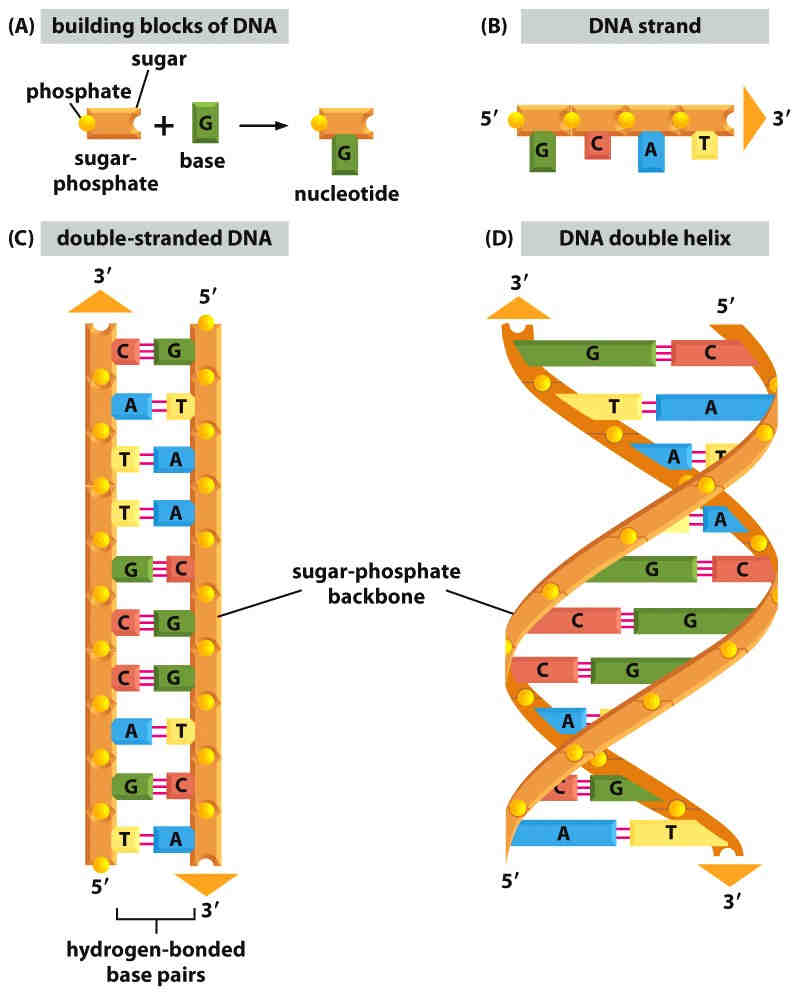
\includegraphics{dna}}
\end{center}
\caption{The structure and composition of DNA. Diagram taken from "Essential Cell Biology" \cite{albertsessential}.}
\label{dna}
\end{figure}

The reciprocal bonding relationships between bases is what allows replication to occur; a copy of the DNA can be made by simply allowing the correct bases to bond to one of the strands making up its helix. This gives a model for inheritance and cellular replication. However, there remains the question of how DNA can actually code for protein. Proteins are made up amino acids bonded in a specific sequence \cite{albertsessential}. The DNA must therefore code for amino acids. This code, which can be thought of as the `digital' representation for the `analogue' protein used by our cells, needs to be carried to ribosomes which translate it into protein \cite{albertsessential}. This is a task carried out by Ribonucleic Acid (RNA). RNA is very much like DNA in that it can bond reciprocally to another strand with matching bases. The main difference is that it is single stranded in structure, and has Uracil (U) in place of Thymine \cite{albertsessential}. It is important to note that in RNA molecules G and U pairings are also possible. RNA bonds to DNA and, in a sense, reads it. This results in the production of a copy of the DNAs genetic payload. This `downloaded' information is then carried away to be translated into protein \cite{albertsessential}. An example of this is depicted in Figure \ref{transcription}, in which we see a Messenger RNA molecule bonding to and thus making a copy of a section of DNA. As depicted in Figure \ref{transcription}, the 3' end of a DNA or RNA molecule is the end onto which new nucleotides are added. The 5' end is chemically stable, and nucleotides are not usually appended to it \cite{albertsessential}.

\begin{figure}
\begin{center}
\scalebox{0.23}{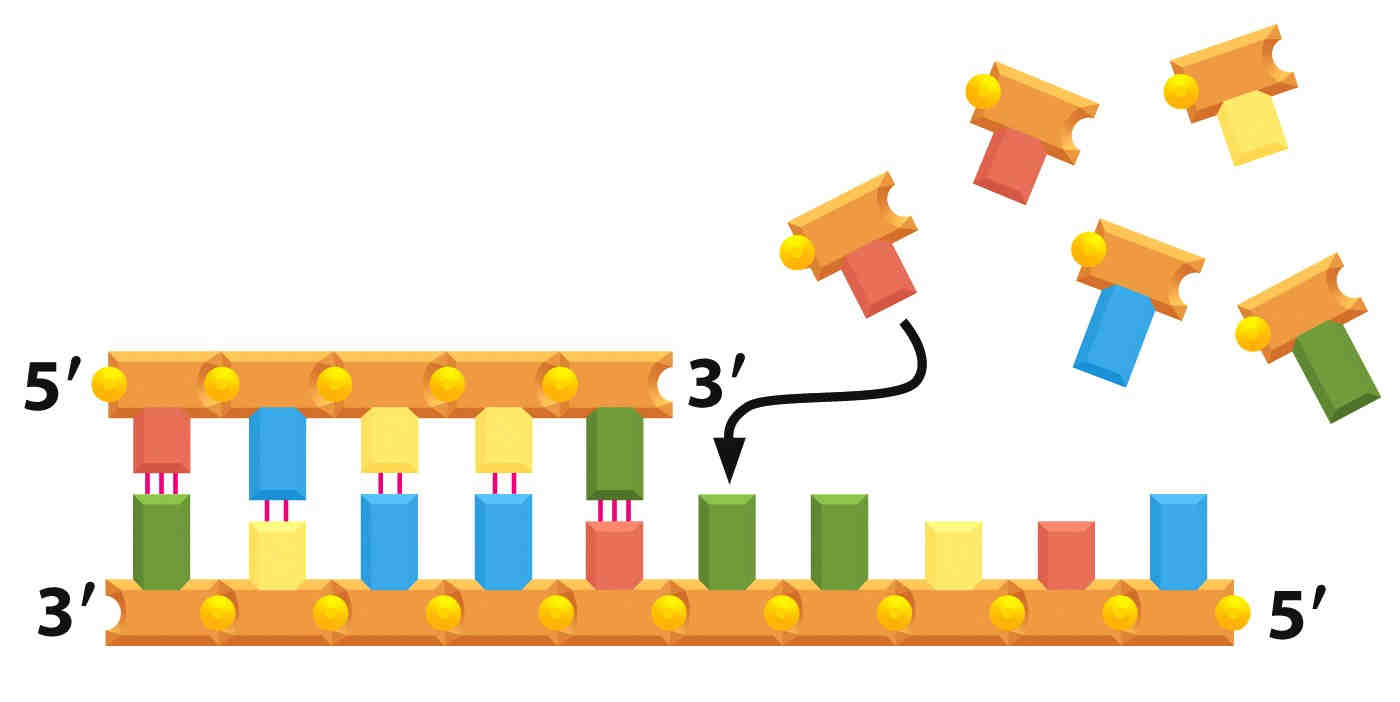
\includegraphics{transcription}}
\end{center}
\caption{RNA transcription. Diagram taken from "Essential Cell Biology" \cite{albertsessential}.}
\label{transcription}
\end{figure}



For many years the conventional wisdom was that DNA contained genes which coded for functional proteins used by the cell \cite{albertsessential}. Though this is undoubtedly true, there was a problem: much of the human genome, and the genomes of other species, contains DNA which does not appear to code for anything \cite{beaton1999eukaryotic}. Many theories have been put forward to explain this. It was argued that this `junk' DNA is the perennial build-up of mutation, and that natural selection simply cannot act with strong enough selective force to cull this free-loading DNA \cite{beaton1999eukaryotic}. Surprisingly, much of this non-coding DNA is actually transcribed into RNA, despite having no apparent function \cite{leung2013coral}. As it turns out, RNA is more than a simple messenger for encoded proteins. Recent research has found myriad important functions for RNA. For example, RNA can act as a catalyst for RNA splicing and peptide bond formation, and can also alter the regulation of genes \cite{xu2012statistical}. It seems that much of our genome contains templates for non-coding RNAs (ncRNAs). These RNAs perform essential cellular functions without actually being translated into protein at any point in their life-cycle \cite{leung2013coral}. Because of its inherently single stranded nature, RNA forms bonds with itself, folding into secondary and tertiary structures \cite{conn1998rna}.


It is axiomatic that chemical structure is tantamount to biological function; RNA is no exception. For this reason there has and continues to be an intense interest in predicting the secondary structure and tertiary structure of RNA molecules. This is in part because it will elucidate the underlying principles of RNA structure formation and function \cite{conn1998rna}, but also because it will allow the detection and classification of unknown RNAs, enable prediction of novel RNA function, and assist the design of new RNA based drugs \cite{condon2003problems}. In fact, RNA is an extremely versatile molecule, and as such is attractive from both an engineering and computational point of view. Small combinatorial computation problems have been solved by representing the solution set using RNAs. Furthermore, a theory of computation has been put forward using self assembling RNA molecules \cite{condon2003problems}. As if to comment on the upheaval of a protein-centric view of biology in recent years, researchers have found that RNA is capable of supporting all the processes required for life without the need of protein \cite{condon2003problems}. The secondary structure of RNA is also highly conserved during evolution, indicating its importance \cite{hofacker2008rna}. Secondary and tertiary structures can be treated hierarchically, as a result it is possible to predict the secondary structure of an RNA without understanding the tertiary structure. The tertiary structure in turn builds upon the secondary structure \cite{tinoco1999rna}. This paper will focus on secondary structure prediction.

It holds to reason that an algorithm for RNA secondary structure prediction can never be realised if we do not understand how these structures form, or their general morphology. For this reason it is important to understand how true RNA secondary structures can be determined, and the limitations of these techniques. DNA and RNA molecules can be analysed using X-ray crystallographic methods. These types of approaches work because the wavelengths of some X-rays are the same as the dimensions of DNA and RNA inter-atomic bonds. The diffraction of X-ray light by these molecules can thus be observed and their structures can subsequently be inferred by analysis of the resulting data. Nuclear Magnetic Resonance (NMR) is another technique which can be applied to the analysis of DNA/RNA. It relies on the spin of atoms when in a magnetic field. These spin signals can be used to determine the atomic composition and topology of a molecule. This has the advantage of not requiring the molecule under analysis to be crystallized before analysis. Arguably this gives a better in vivo view of RNAs/DNAs, which are fundamentally flexible structures. NMR also has some disadvantages; for instance, it is less accurate than X-ray crystallography, and cannot be used on extremely large molecules. The reason these techniques cannot be used for all RNA structural assays is that they are extremely expensive and time consuming \cite{neidle2010principles}.


RNA secondary structure prediction techniques can be broadly broken into two categories: those that use auxiliary information to assist in prediction, and those that predict structure ex nihilo---that is, with nothing but the `proband' sequence we require a structure for. The former approach typically does consensus matching between some sequences for which a user already knows the secondary structures, and a sequence for which the structure is unknown \cite{hofacker2008rna}. In this paper I investigate the latter approach because it requires deeper knowledge about why and how RNAs fold. Also, it is the more general of the two.



\section{Getting Started}

The {\tt cshonours} files are located in:
\begin{verbatim}
/cslinux/cstex/local
\end{verbatim}

In order to use the {\tt cshonours} class you need to tell \TeX\ how
to find it. To do this simply add the following to your shell resource
file (ie.\ {\tt .zshrc}, {\tt .bashrc}, etc):
\begin{verbatim}
export TEXINPUTS=$TEXINPUTS:.:/cslinux/cstex//
\end{verbatim}
(The double-slash \verb!//! tells \TeX\ to search the tree from this
point.) Then open a new shell window to run \LaTeX\ in.

If you are using a machine that doesn't mount {\tt cslinux} or a
stand-alone system such as a home machine, you can take a copy of the
{\tt cshonours.cls} file and put it on your own machine. Please copy
the class file directly from the original in the above directory to
make sure you have an unadulterated copy.

Once you have told \TeX\ how to find the class file, the easiest way
to get started is to copy this example file, {\tt cshonours.tex}, and
the accompanying example bibliography file, {\tt cshonours.bib}, from
the above directory, give them a new name, and start modifying the text.

\section{What does it all mean?}
\label{code}

The example file is pretty self explanatory, but here's a little
elucidation for those who are interested.

\begin{verbatim}
\documentclass{cshonours}
\end{verbatim}
\ldots tells \LaTeX\ to use the {\tt cshonours} class. The commands
between here and the \verb!\begin{document}! command are known as the
{\em preamble\/} of the latex document. Font size is automatically set
to 12pt in this class.

\begin{verbatim}
\bibliographystyle{acm}
\end{verbatim}
\ldots sets the bibliography style. Default is the style used in
Transactions of the ACM.

\begin{verbatim}
\usepackage{graphics}  %optional
\end{verbatim}
\ldots this is only needed if you want to include postscript images.

\begin{verbatim}
\title{The Honours Dissertation Class for \LaTeX2e}
\author{Cara MacNish}
\end{verbatim}
\ldots same as usual.

\begin{verbatim}
\keywords{Honours, report preparation, \LaTeX}
\categories{A.2, I.7.2}
\end{verbatim}
\ldots keywords and Computing Reviews classification numbers. These
will be put at the bottom of the abstract page.

\begin{verbatim}
\begin{document}
\end{verbatim}
\ldots so much for the preamble, now we start the document proper.

\begin{verbatim}
\maketitle
\end{verbatim}
\ldots produces the title page using the title and author stored
earlier. Unlike the standard {\tt report} class it also starts roman
page numbering.

\begin{verbatim}
\begin{abstract}
This is a short report...
\end{abstract}
\end{verbatim}
\ldots produces the abstract page, including the keywords and
categories stored earlier.

\begin{verbatim}
\begin{acknowledgements}
This style is designed...
\end{acknowledgements}
\end{verbatim}
\ldots produces the acknowledgements page.

\begin{verbatim}
\tableofcontents
\listoftables  %optional
\listoffigures  %optional
\end{verbatim}
\ldots you guessed it! \verb!\listoftables! and \verb!listoffigures!
can be omitted if you have no tables or figures respectively.

\begin{verbatim}
\chapter{The Honours Dissertation Style Guide}
\end{verbatim}

\ldots and so the first chapter begins. Unlike the standard {\tt
report} class the first \verb!\chapter! command also switches
pagenumbering to arabic.

The main body is created using the usual \LaTeX\ commands. At the end
we come to:

\begin{verbatim}
\appendix
\end{verbatim}
\ldots starts off the appendices.

\begin{verbatim}
\bibliography{cshonours}
\end{verbatim}
\ldots puts in the bibliography, generated in this case from the
file {\tt cshonours.bib}.


\section{Carrying on\ldots}

The rest of the document proceeds in the usual way, with all standard
\LaTeX\ commands available. These are described in~\cite{bible}, which
is written by the author of \LaTeX, Leslie Lamport, and commonly known
as the \LaTeX\ ``Bible''.

For those who are feeling ambitious, a wealth of contributed
packages, some of which are included in our distribution, and some of
which you would need to download yourself, are described
in~\cite{doggie}, commonly known as the ``Doggie Book''.


\section{Including Postscript Files}

Most drawing packages (such as {\tt xfig} and {\tt xpaint}) and image
manipulation packages (such as {\tt xv} and {\tt gimp}) allow you to
save your work as (encapsulated) postscript, which can be easily
included in your \LaTeX\ document. The recommended (and simplest!) way
of doing this is by including the command \verb!\usepackage{graphics}!
in the preamble (see Section~\ref{code}) and then include the
postscript file using the \verb!\includegraphics! command.

\begin{figure}
\begin{center}

\includegraphics{gnu}
\end{center}
\caption{This is a Gnu.}
\label{gnu}
\end{figure}

For example, Figure~\ref{gnu} shows a Gnu, produced by the following code:
\begin{verbatim}
\begin{figure}
\begin{center}

\includegraphics{gnu}
\end{center}
\caption{This is a Gnu.}
\label{gnu}
\end{figure}
\end{verbatim}

\begin{figure}
\begin{center}
\scalebox{0.6}{
\includegraphics{gnu}}
\end{center}
\caption{This is a smaller Gnu.}
\label{smallergnu}
\end{figure}

You can scale graphics using the \verb!\scalebox! command. For
example, Figure~\ref{smallergnu} shows a smaller Gnu, produced as follows:
\begin{verbatim}
\begin{figure}
\begin{center}
\scalebox{0.6}{
\includegraphics{gnu}}
\end{center}
\caption{This is a smaller Gnu.}
\label{smallergnu}
\end{figure}
\end{verbatim}


\section{Producing Postscript Output}

\LaTeX\ produces a {\tt .dvi} file which you can convert to postscript
using {\tt dvips}. If you have included encapsulated postscript figures the
bounding boxes of those figures sometime confuse the printing
routines. To overcome this it is recommended you use the {\tt -K}
option to strip bounding box comments out. The full recommended format
is:

\begin{verbatim}
dvips -K -f myfile.dvi > myfile.ps
\end{verbatim}

To save typing I just use a simple script for
all my {\LaTeX}ing. Just create a file, called say {\tt laps}, containing something like:
\begin{verbatim}
latex $1
dvips -K -o $1.ps $1.dvi
\end{verbatim}
Then make it executable, run \LaTeX\ with the command
\begin{verbatim}
laps myfile
\end{verbatim}
and view with ghostview (with ``State'' set to ``Watch file'').

\section{Producing PDF}

If you prefer PDF output you can produce this using {\tt
pdfelatex}. This does not use {\tt dvi} as an intermediary so you just
say:
\begin{verbatim}
pdfelatex myfile
\end{verbatim}

Note that any graphics you include must also be in
suitable PDF. There are conversion programs, such as {\tt ps2pdf}, but
I've found they often don't work well. It is better to produce the
graphics directly in {\tt pdf}.

I've also found that {\tt pdf} viewers don't tend to refresh well, so
that you need to keep opening the file. As a result I tend to
postscript where possible.


\section{Emacs and \LaTeX}

Gnu Emacs and Xemacs recognise both {\tt .tex} and {\tt .bib} files,
and provide a number of tools for preparing them. For example you can
select {\tt .bib} entry templates from a drop-down menu. Simple
commands like \verb!C-c C-e! (puts in the \verb!\end! command to
finish an environment) save lots of typing.


\section{Appendices}

After the main body comes the appendices. See Appendix~\ref{appa} and
Appendix~\ref{appb}.

\section{Bibliography}

Finally, the bibliography can be produced automatically from a {\tt .bib} file
using {\tt bibtex} in the usual way. This is described
in~\cite{bible}. 

The bibliography is the only change from the \LaTeX 2.09 {\tt
cshonours} style file. The bibliography now comes after the
appendices, in line with printed books, and uses alphanumeric citation
tags to make reading (and marking) easier.


\appendix

\chapter{Original Honours Proposal}
\label{appa}

You must include as your first appendix an exact copy (in wording) of
your original project proposal. This aids other readers to establish
what was the initial focus of the project.

\chapter{Another Appendix}
\label{appb}

Other appendices might include pseudocode 
for your implementation, a Users Manual, an important data file, etc. 

\bibliography{cshonours}

\end{document}


